\chapter{Servidor de imágenes con tecnologías web }\label{cap.camserver}
En este capítulo expondrá la creación de un nuevo driver para la plataforma JdeRobot. Este driver será un servidor de imágenes, al que se ha llamado camServerWeb, obtenidas mediante una webcam (ya sea externa o interna del ordenador) de modo que cualquier aplicación externa pueda obtener las imágenes obtenidas.
\section{Diseño}
Este driver está diseñado con JavaScript y HTML como lenguajes de programación, y ROS como middleware para la interconexión con los diferentes clientes. A continuación se muestra un diagrama del diseño del driver:
\begin{figure}[H]
  \begin{center}
    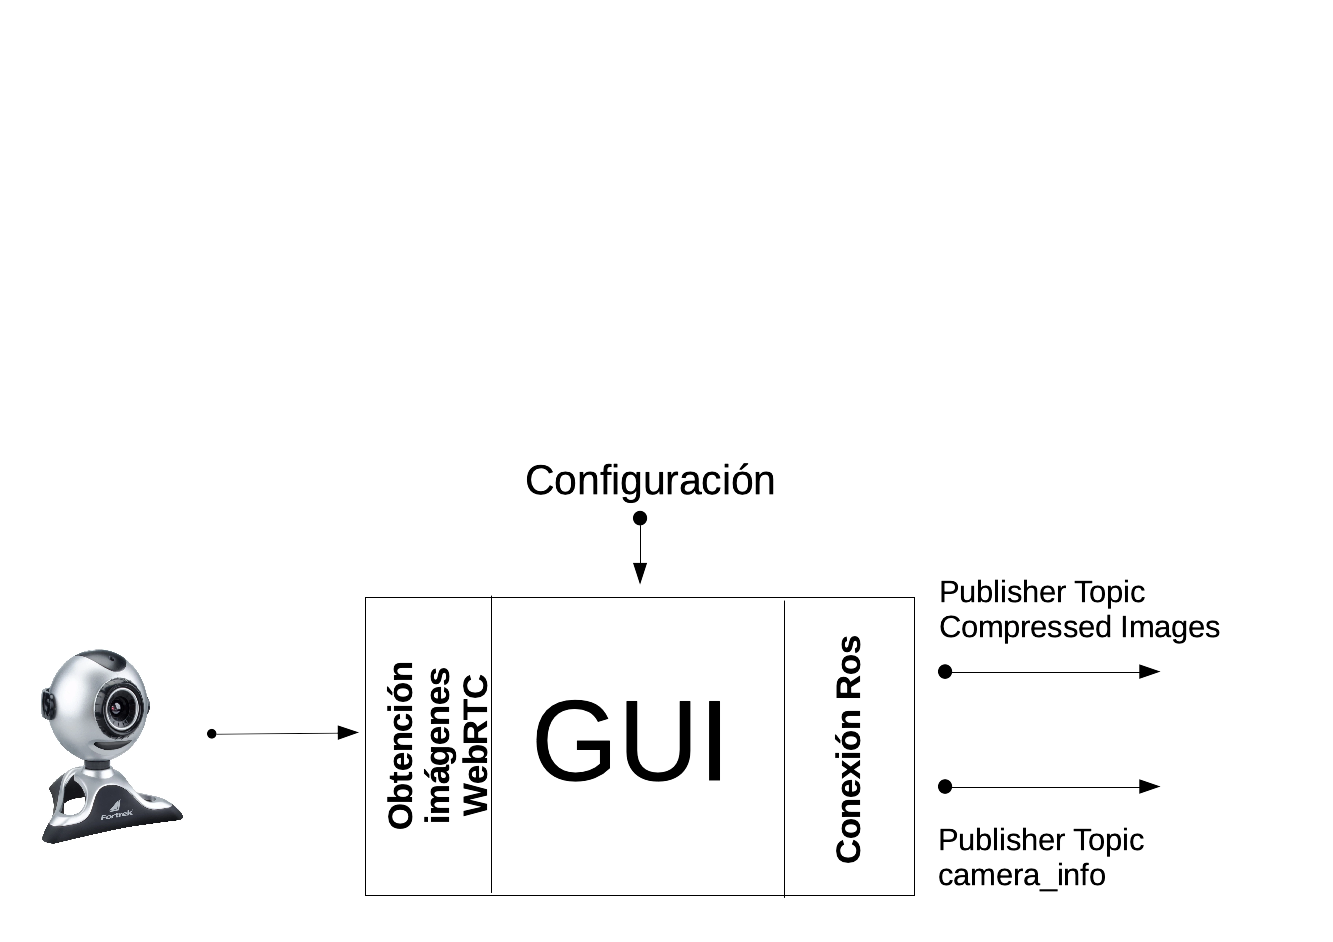
\includegraphics[width=0.8\textwidth]{figures/disenocamserver.png}
		\caption{Diseño del driver camServerWeb}
		\label{fig.diseñocamserver}
		\end{center}
\end{figure}
Como se puede observar, el driver contará con tres partes bien diferenciadas. Una parte será la correspondiente a la interfaz gráfica, que simplemente aportará la configuración del driver, una segunda parte que corresponderá a la adquisición de las imágenes usando WebRTC para realizar la conexión con la fuente de video, y una última parte que será la encargada de realizar la conexión mediante ROS y el posterior envío de los mensajes mediante los Publisher de ROS.

\section{Configuración}
Para configurar el driver, se ofrecen dos posibilidades:
\begin{itemize}
\item Mediante el uso de un fichero con formato``YAML'' al igual que en resto de herramientas de este trabajo. 
\item Mediante el menú de configuración incorporado en la interfaz gráfica.
\end{itemize}
El primer método realiza la configuración inicial del driver, ya que se configura al ejecutar el driver. El segundo método permite realizar la configuración del driver durante la ejecución del mismo, ofreciendo la posibilidad de que no sea necesario cerrar y tener que volver a lanzar el driver cada vez que se quiera reconfigurarlo.

Los parámetros configurables son los siguientes:
\begin{itemize}
\item Dirección IP. Por defecto será ``localhost''
\item Puerto. Por defecto será ``9090''
\item Topic al que se deberán registrar los clientes. Por defecto será ``/usb\_cam/image\_raw/compressed''
\item Formato del mensaje. Por defecto será ``sensor\_msgs/CompressedImage''
\item Framerate. Por defecto serán 20 fps
\item Fuente de video. Por defecto será la primera fuente detectada por WebRTC. Este parámetro únicamente puede ser configurado mediante el menú de configuración de la interfaz gráfica.
\end{itemize}

\subsection{Interfaz gráfica}
La interfaz está realizada mediante HTML y Bootstrap, siguiendo el modelo del resto de aplicaciones web de la plataforma JdeRobot.
\begin{figure}[H]
  \begin{center}
    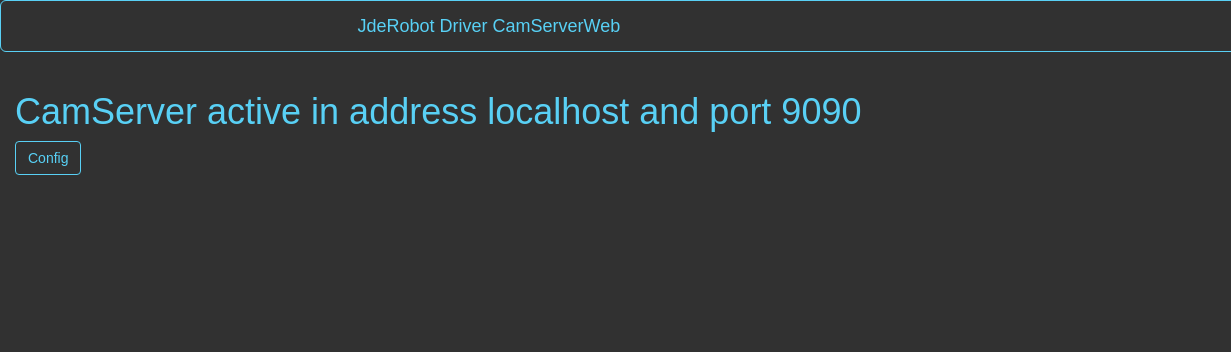
\includegraphics[width=0.8\textwidth]{figures/Interfazcamserver.png}
		\caption{Interfaz gráfica del driver}
		\label{fig.interfazcamserver}
		\end{center}
\end{figure}
La configuración se realizará gracias a un menu desplegable mediante la pulsación de un botón y una vez que se pulse el botón guardar, se almacenarán la nueva configuración para realizar las conexiones que se explicarán en las siguientes secciones:
 \begin{figure}[H]
  \begin{center}
    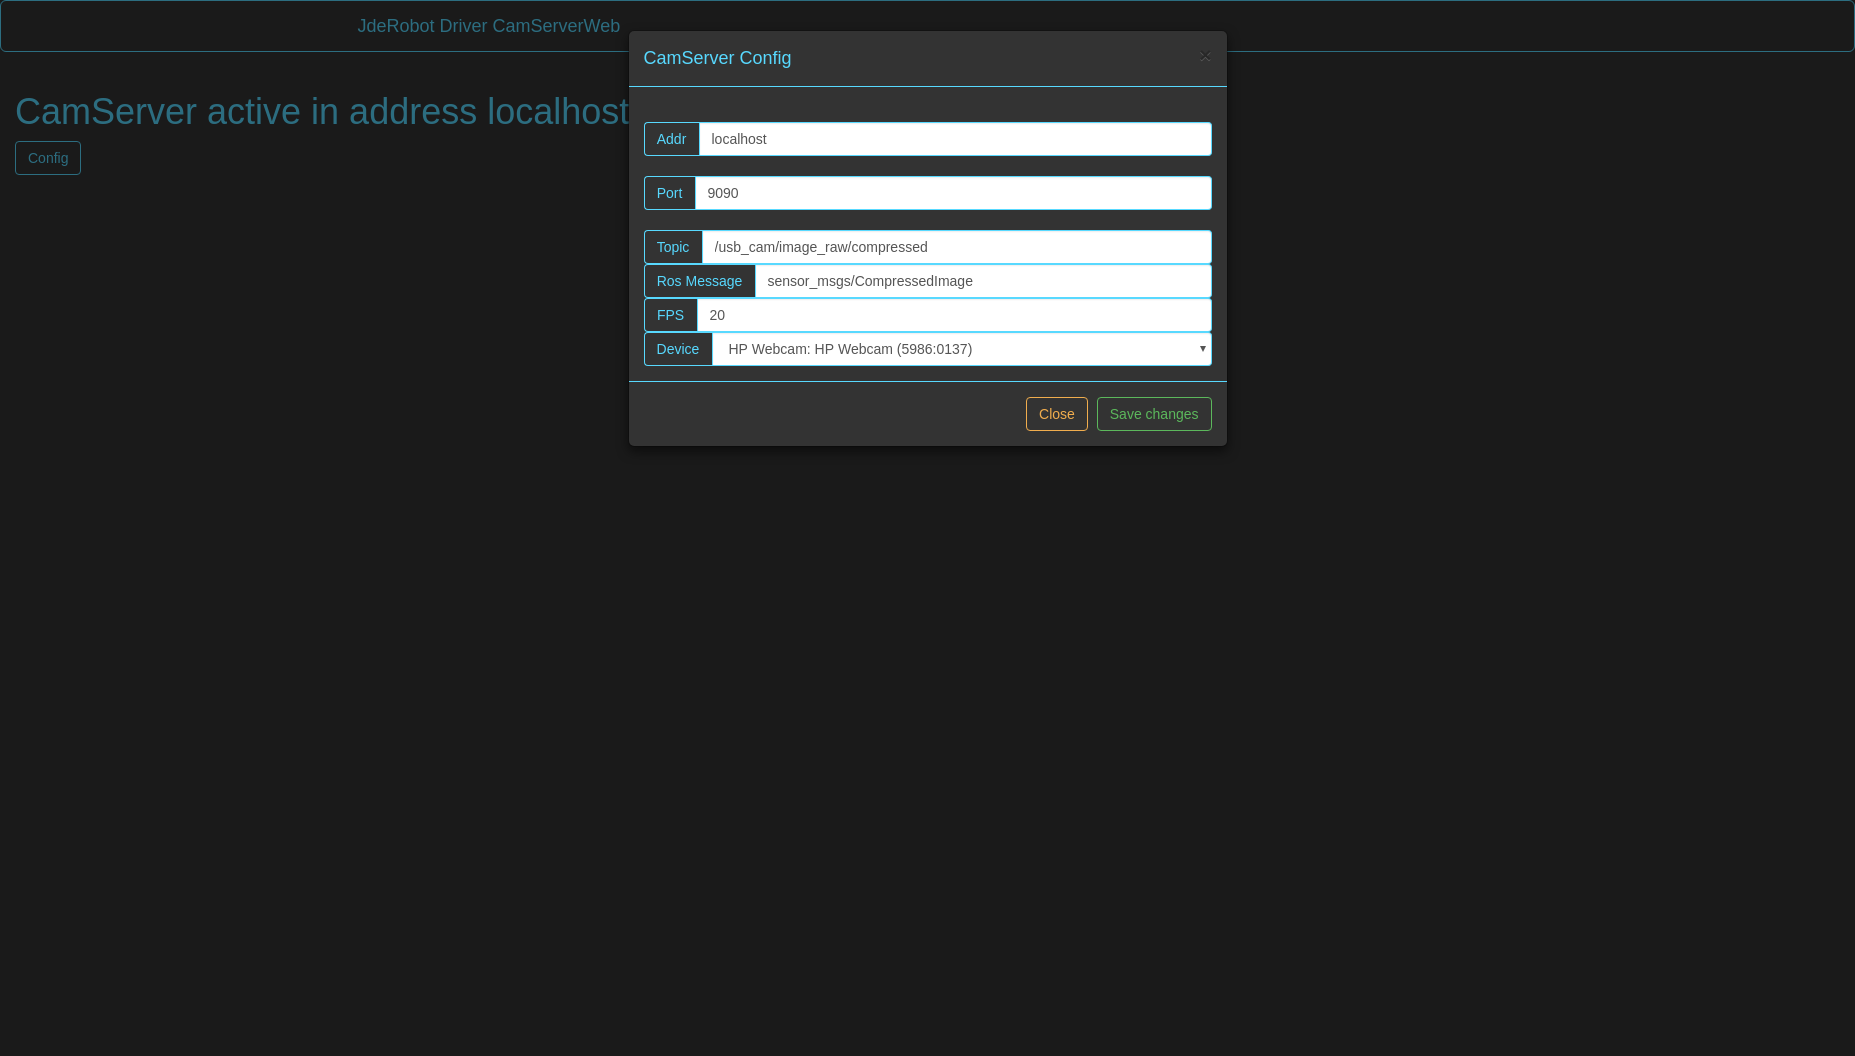
\includegraphics[width=0.8\textwidth]{figures/configcamserver.png}
		\caption{Menú de configuración del servidor de imágenes}
		\label{fig.configcamserver}
		\end{center}
\end{figure}

\section{Adquisición de las imágenes}
Para la obtención de las imágenes, como se ha indicado anteriormente, se hace uso del proyecto de código abierto webRTC, que nos permite la transmisión en tiempo real de audio, video y datos.
Mediante webRTC, obtenemos las imágenes de una cámara utilizando muy pocas línea de código, lo que nos facilita enormemente el trabajo. El único problema que se ha tenido que tener en cuenta y solucionar, es el formato en el que se obtienen esas imágenes que es incompatible con ROS, por lo que se han tenido que llevar a cabo modificaciones en el formato de la imagen.

Lo primero que se debe realizar es recopilar todos los dispositivos conectados al ordenador y separar los dispositivos de video, que son los que realmente nos interesan. Para lograrlo, se utiliza el api Navigator de webRTC, proporcionándonos el objeto navigator.mediaDevices, al cual si le añadimos .enumerateDevices().then(function (devices)\{\}, obtenemos todos los dispositivos multimedia conectados al ordenador donde se está ejecutando. Una vez que ya tenemos todos los dispositivos, simplemente nos interesan como se ha indicado anteriormente, aquellos dispositivos capturadores de video, es decir serán aquellos dispositivos cuyo tipo es de entrada de video (en nuestro código sería un condicional if (devices.kind == "videoinput")\{\}). La lista de dispositivos se mostrará en el menu de configuración, mostrado en la sección anterior, mediante un campo desplegable como se muestra en la siguiente imagen:
 \begin{figure}[H]
  \begin{center}
    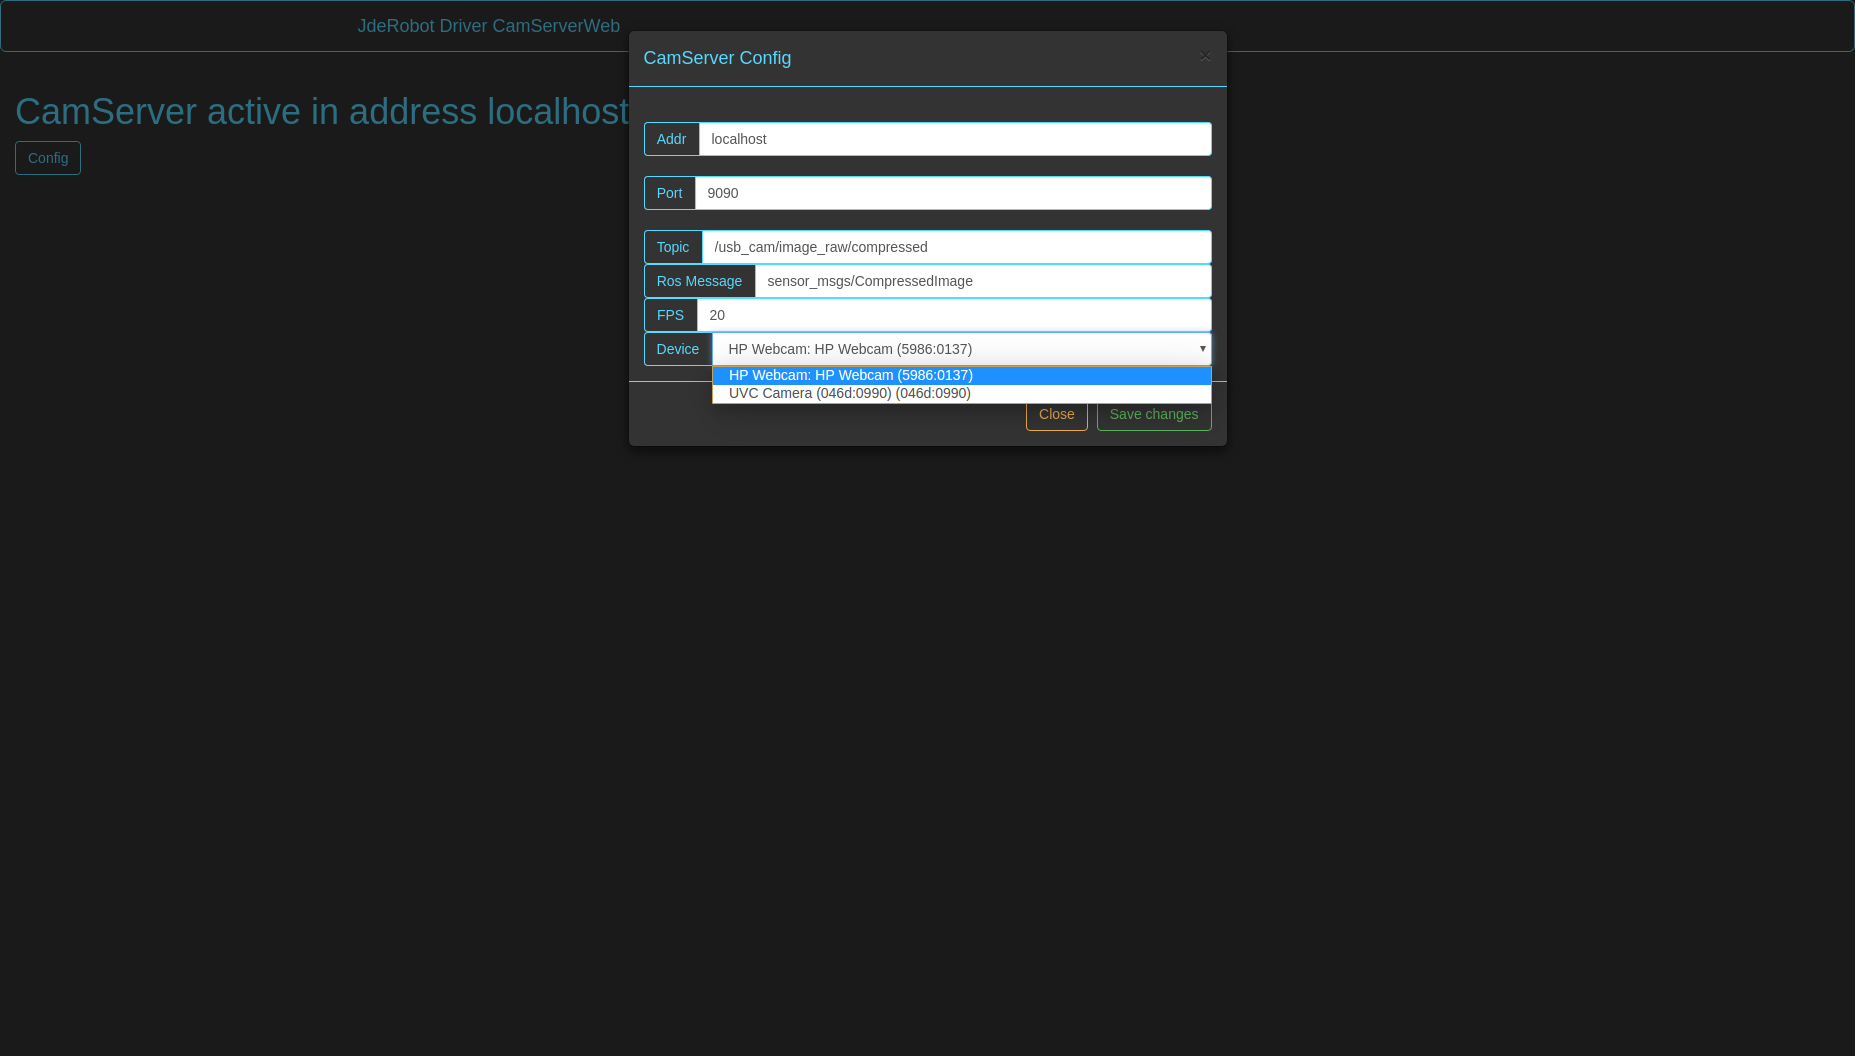
\includegraphics[width=0.8\textwidth]{figures/devicecamserver.png}
		\caption{Selector del dispositivo de entrada de video}
		\label{fig.devicecamserver}
		\end{center}
\end{figure}
Una vez que seleccionamos el dispositivo que vamos a utilizar para adquirir las imágenes, hay que conectarse a él. Para esta conexión, volvemos a utilizar la API de webRTC, Navigator y el objeto Navigator.mediaDevices, sin embargo en esta ocasión utilizamos el método navigator.mediaDevices.getUserMedia(constraints).then(function(stream) \{\}), donde constraints define los dispositivos multimedia (en este caso el dispositivo de entrada de video escogido) y stream es el flujo de datos obtenido de ellos.
Este flujo de datos está en el formato MediaStream, el cual no es apto para ser enviado o visualizado, por tanto es necesario realizar una reconversión. Para realizar la reconversión, vamos a utilizar el elemento de HTML canvas y el método JavaScript asociado a este elemento toDataURL(). Este método nos devuelve un data URI (URLs prefijados que permiten a los creadores de contenido incorporar pequeños archivos en línea en los documentos) que contiene una representación de la imagen en el formato especificado por el parámetro type, tomando en nuestro caso el valor "image/jpeg", para obtener las imágenes en el formato comprimido jpeg. Todo esto estará contenido en un canvas virtual, ya que no se mostrará en ningún lugar y únicamente se utilizará como pasarela entre el API de webRTC y el envío de las imágenes.

\section{Conexiones}
En esta sección se explicará cómo realizar la  conexión a ROS y el posterior envío de imágenes mediante un Publisher de ROS. Como se indica en los capítulos anteriores, dado la limitación y la política de privacidad las tecnologías web, es necesario la existencia de un servidor intermedio que estará escuchando en una dirección IP y en un Puerto determinado, y hará las funciones de control de acceso y encaminamiento.

\subsection{Establecer conexión}
Para realizar la conexión es necesario el uso de la biblioteca roslibjs y que se ha explicado en capítulos anteriores. Esta biblioteca nos proporciona todo el código necesario para realizar la conexión, indicándonos si se ha realizado correctamente o a si ha ocurrido algún error. Para realizar la conexión, la biblioteca roslibjs nos proporciona el objeto ROSLIB.Ros, y el método proporcionado por este objeto, ros.on. El código para establecer la conexión queda como sigue:
\begin{lstlisting}[frame=single]
ros = new ROSLIB.Ros();
ros = new ROSLIB.Ros({
            url : "ws://IP:Puerto"
 });
\end{lstlisting}
En este código, indicaremos que la conexión se hará utilizando un canal de comunicación WebSocket, y la IP y puerto por la que se transmitirá. De esta forma ya habremos establecido la conexión ROS, pero aún deberemos definir el tipo de mensaje a enviar y a través de que etiqueta de ROS (topic de ROS) nos pueden localizar los clientes que deseen obtener lo que nuestro servidor de imágenes está transmitiendo.

\subsection{Mensajes}

\subsubsection{Definición de la estructura de los mensajes}
El tipo de mensaje que vamos a utilizar para el envío será el tipo predefinido en el API de ROS, "sensor\_msgs/CompressedImage". El motivo de la elección de este tipo es debido a que las imágenes se obtienen en formato comprimido "jpeg", tal y como se ha explicado en la sección anterior. Sin embargo, este tipo de mensaje no envía información acerca del tamaño de la imagen (altura y anchura), por lo que es necesario enviar otro mensaje adicional para completar esta información. Este mensaje de apoyo será de tipo "sensor\_msgs/CameraInfo" y transmitirá toda la información sobre la cámara (frames por segundo, altura, anchura, etc). Para definir estos dos mensajes, se utiliza el objeto proporcionado por la biblioteca roslibjs, ROSLIB.Topic. A este objete se le deben introducir como parámetros el objetos ROSLIB.Ros generado para realizar la conexión, el nombre del topic y el tipo de mensaje, por lo que generaremos nuestro Publisher para servir las imágenes y la información de la cámara mediante el siguiente código:
\begin{lstlisting}[frame=single]
var imagenTopic = new ROSLIB.Topic({
	ros:ros, 
	name: config.Topic, 
	messageType : "sensor_msgs/CompressedImage Message"})
	
var cameraInfo = new ROSLIB.Topic({
         ros: self.ros,
         name : "/usb_cam/camera_info",
         messageType: "sensor_msgs/CameraInfo"
       })

\end{lstlisting}

\subsubsection{Creación de los mensajes y publicación}
Definidos los mensajes y establecida la conexión, el siguiente paso es transmitir los mensajes. Para ello se deben crear los mensajes con la información que deseamos transmitir con el Publisher, utilizando de nuevo un objeto definido en la biblioteca roslibjs, new ROSLIB.Message. Para crear este objeto, debemos pasar por parámetros el contenido que queramos que tenga nuestro mensaje, siempre cumpliendo las especificaciones definidas para cada tipo de mensaje escogidos anteriormente y que están definidas en la documentación de ROS  \footnote{\url{http://wiki.ros.org/common_msgs}}. En nuestro caso, para definir los dos mensajes que transmitiremos lo haremos mediante el siguiente código para el caso de la transmisión de las imágenes:
\begin{lstlisting}[frame=single]
 var videomensaje = new ROSLIB.Message({
 	format : "jpeg", 
	data : data.replace("data:image/jpeg;base64,", "")
	})

\end{lstlisting}
De el anterior código cabe destacar que data corresponde a los datos obtenidos mediante el método toDataURL indicado anteriormente, remplazando la cabecera donde se indica el formato, ya que el formato ya se indica en el propio mensaje mediante format.  Para el mensaje donde se transmite la información de la cámara usaremos el siguiente código:

\begin{lstlisting}[frame=single]
var camarainfo = new ROSLIB.Message({
	height: imagen.height,
	width: imagen.width})

\end{lstlisting}
Creados los mensajes, solo falta publicarlos, lo que se consigue de una manera sencilla mediante:
\begin{lstlisting}[frame=single]
imageTopic.publish(imageMessage);
cameraInfo.publish(infoMessage);
\end{lstlisting}
Se puede apreciar fácilmente que lo que se está realizando es publicar los dos mensajes creados mediante la estructura definida anteriormente. 
Finalmente, es necesario enviar de una manera periódica estos mensajes, ya que con lo indicado anteriormente, únicamente se está enviando un mensaje de cada. Para crear un envió periódico, se hace uso del método de JavaScript SetInterval(). Este método llama a una función o evalúa una expresión cuando pase un intervalo de tiempo (en milisegundos), que se indica en la llamada al método junto a la función que se quiere ejecutar cuando se cumpla el citado intervalo.

\section{Experimentos}
Como se ha visto anteriormente, el driver puede ejecutarse a través de dos vías: Electron y Node.js. Sin embargo, la preparación para que funcione correctamente es la misma para ambas vías, siendo la única diferencia la forma de ejecutar el driver.
A continuación se muestra un esquema del funcionamiento del driver:
\begin{figure}[H]
  \begin{center}
    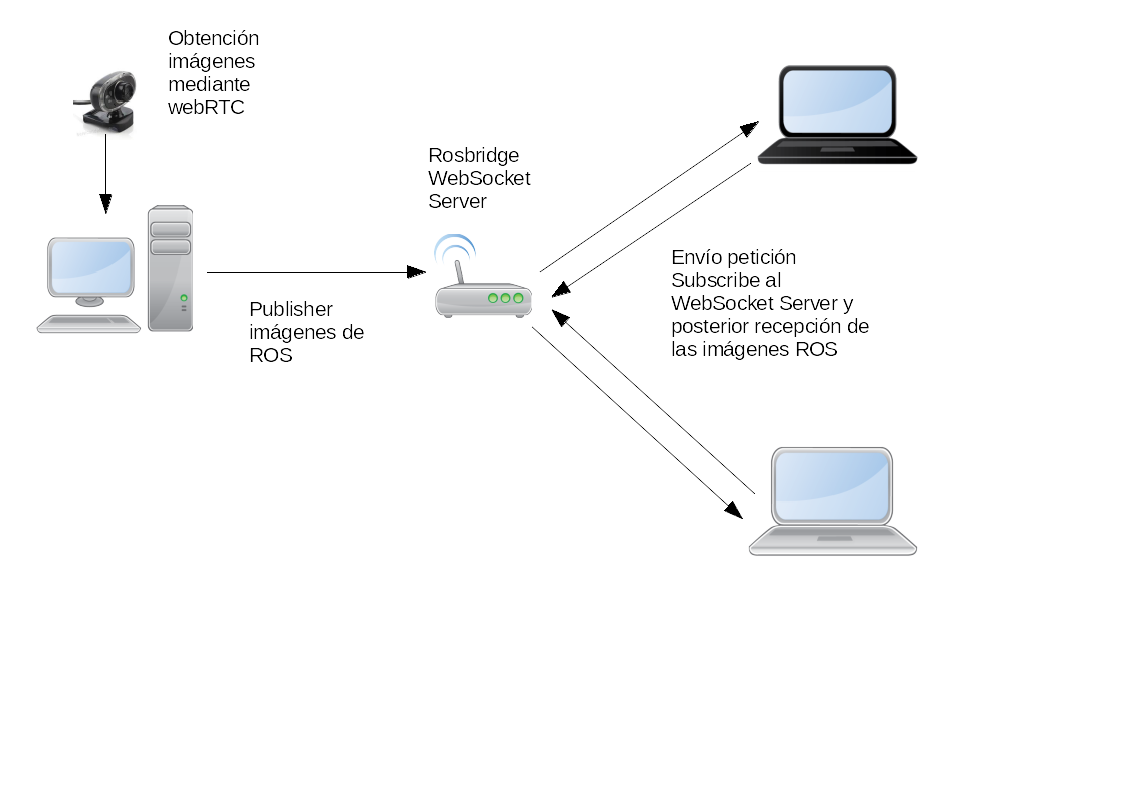
\includegraphics[width=0.8\textwidth]{figures/esquemacamserver.png}
		\caption{Esquema de funcionamiento de camServerWeb}
		\label{fig.esquemacamserver}
		\end{center}
\end{figure}
En un primer terminal o consola se debe ejecutar el servidor intermedio de ROS que se puede ver en el esquema.
\begin{lstlisting}[frame=single]
roslaunch rosbridge_server rosbridge_websocket.launch
\end{lstlisting}
El segundo terminal se ejecutará el driver.
\begin{itemize}
\item 
Con Node.js
\end{itemize}
\begin{lstlisting}[frame=single]
node run.js
Arrancamos nuestro navegador favorito y ponemos la url http://localhost:7777/
\end{lstlisting}
\begin{itemize}
\item 
Con Electron
\end{itemize}
\begin{lstlisting}[frame=single]
npm install
npm start
\end{lstlisting}
En ambos casos debemos configurar el driver para que se conecte con el servidor intermedio, en la imagen 4.5 muestra una posible configuración del driver.
\begin{figure}[H]
  \begin{center}
    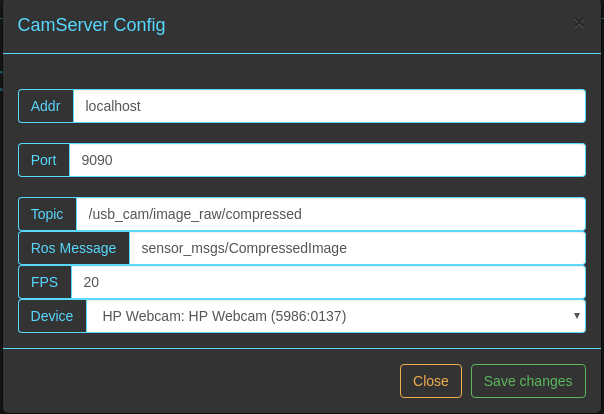
\includegraphics[width=0.8\textwidth]{figures/configcamservertest.png}
		\caption{Ejemplo de configuración del driver}
		\label{fig.esquemacamserver}
		\end{center}
\end{figure}
Finalmente, para verificar que está funcionando correctamente, en un tercer terminal lanzaremos la herramienta rqt\_image\_view, facilitada por ROS para visualizar imágenes enviadas a través de un mensaje de ROS, que hará la función de cliente en nuestro esquema.
\begin{figure}[H]
  \begin{center}
    \subfigure[Node.js]{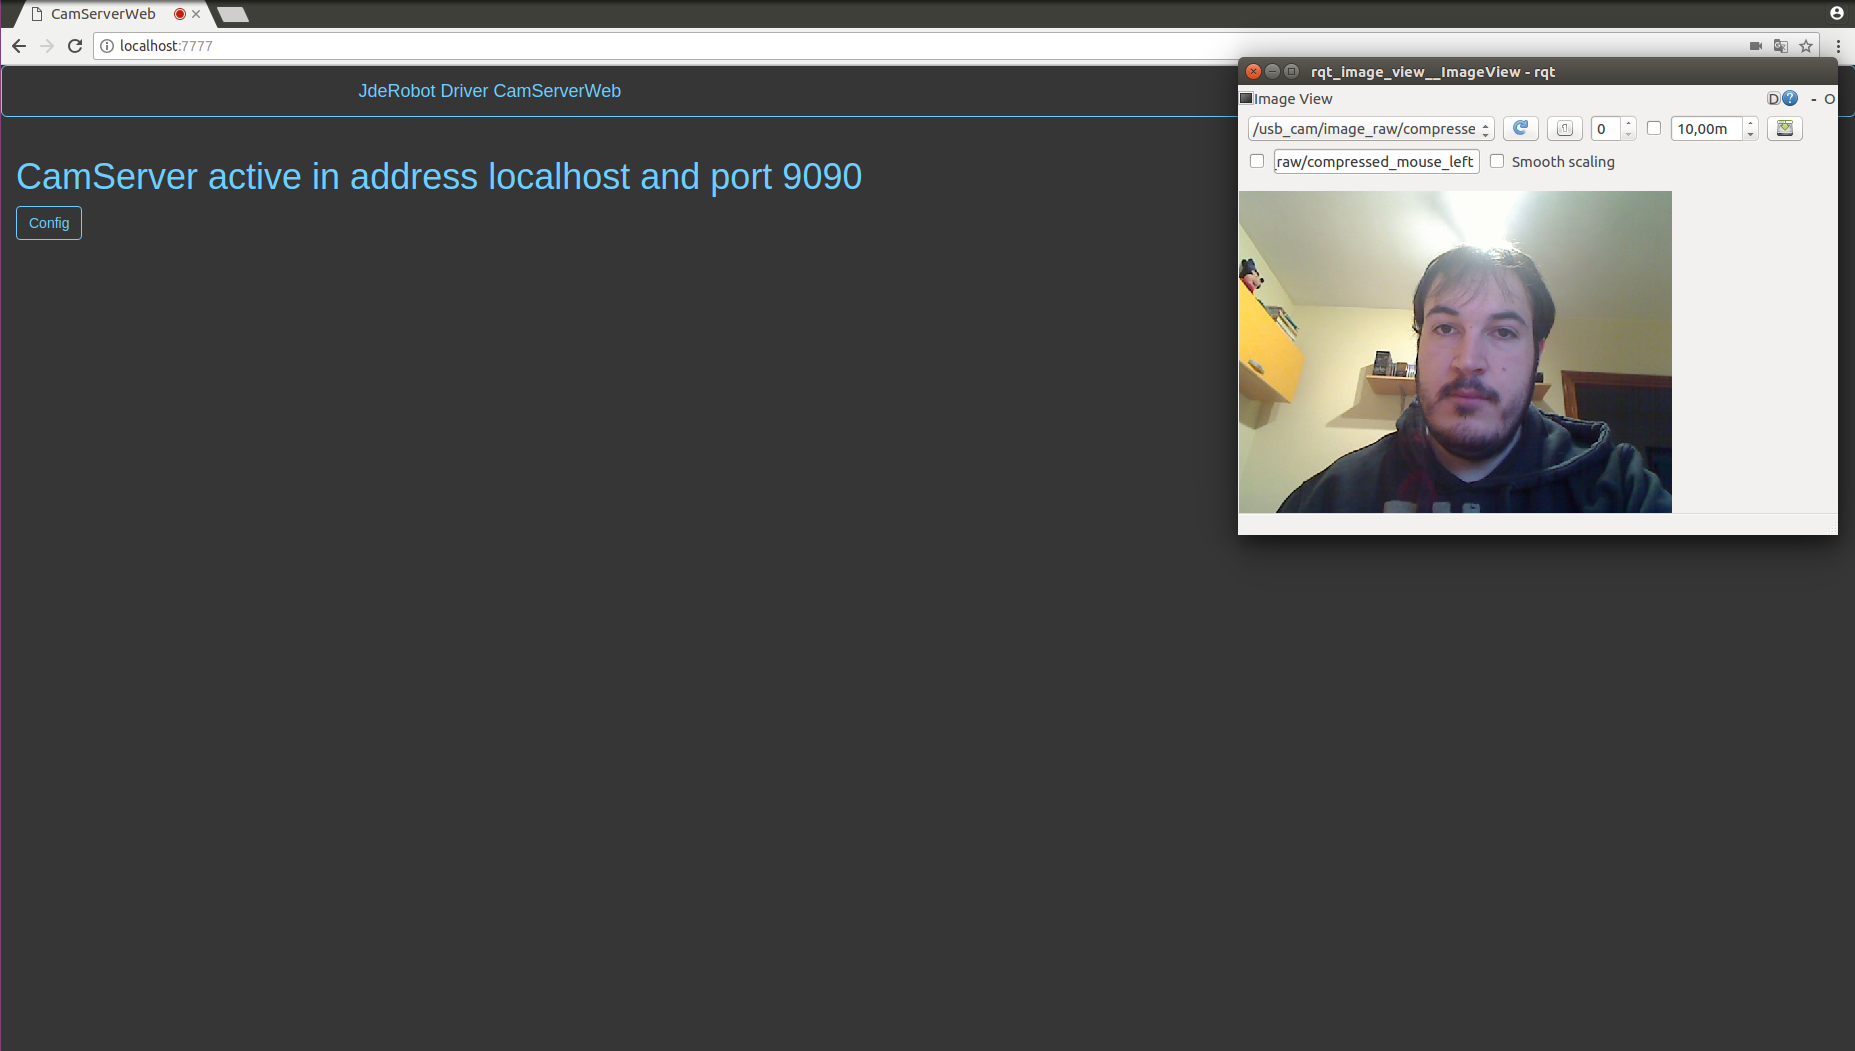
\includegraphics[width=0.4\textwidth]{figures/camservernodejs.png}}
    \subfigure[Electron]{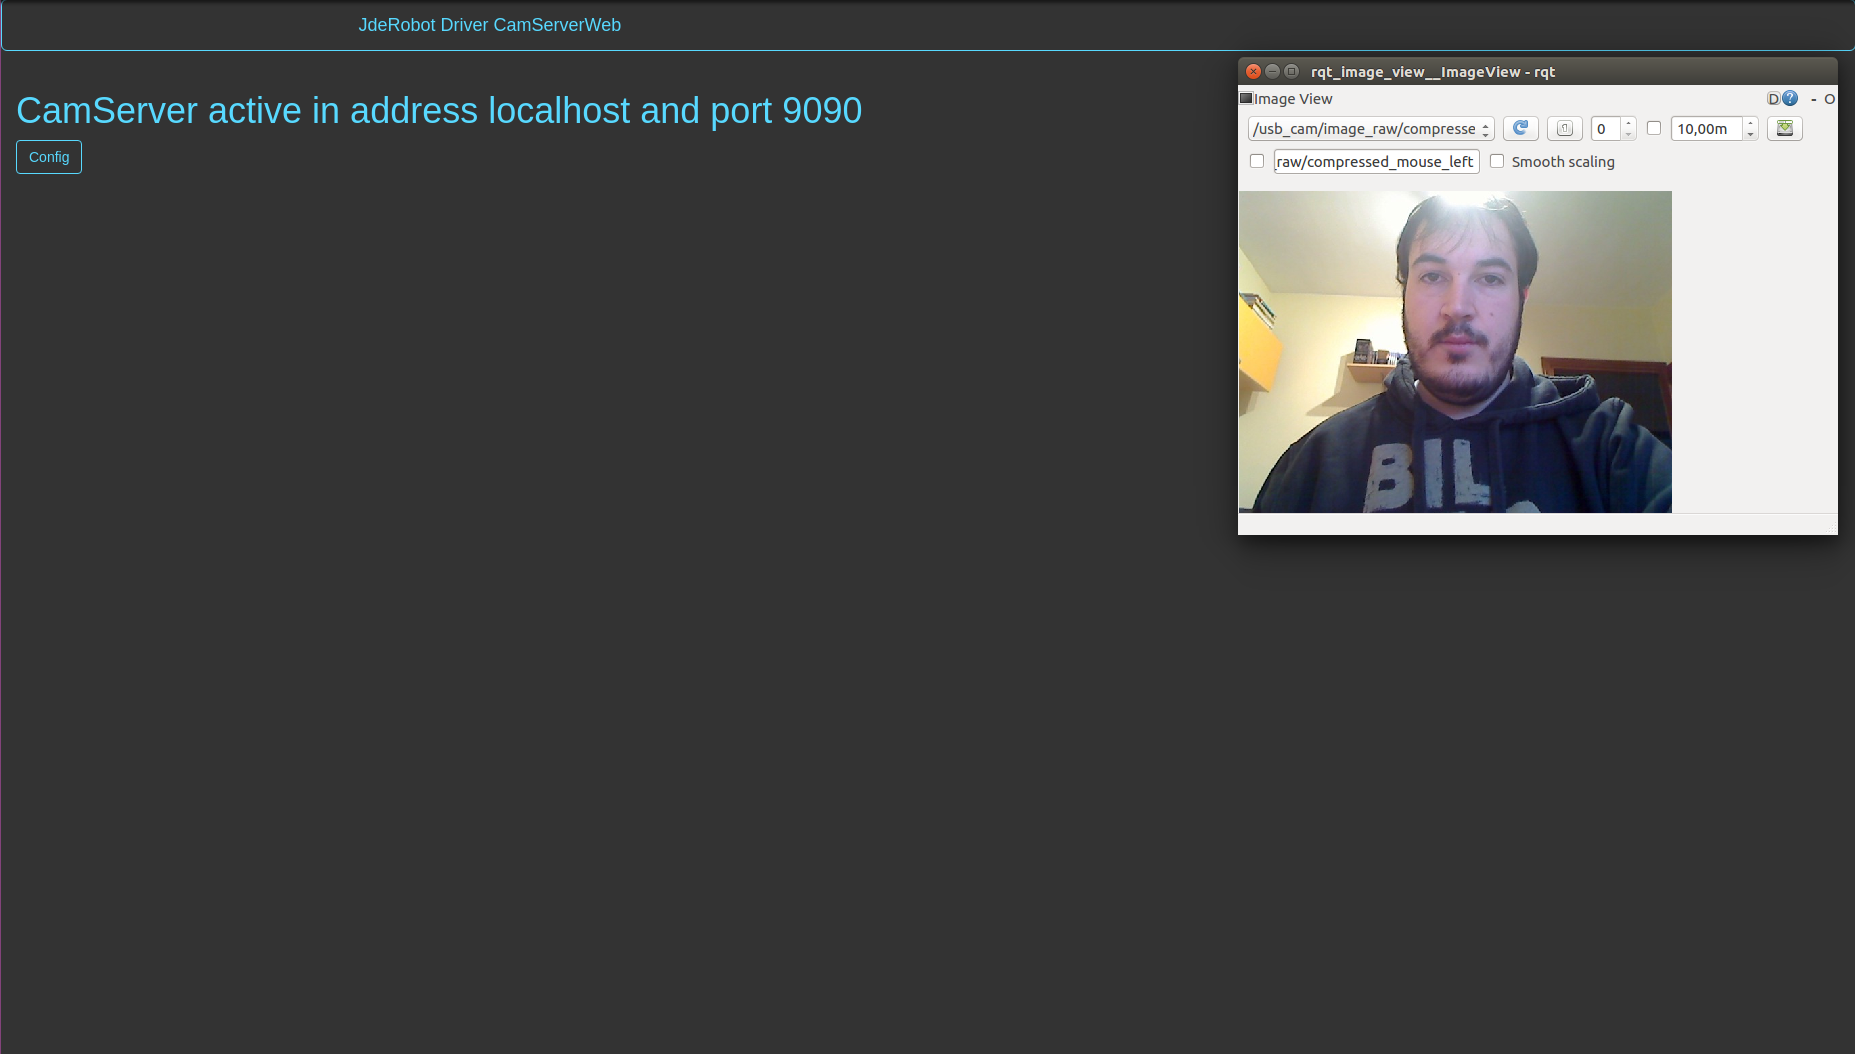
\includegraphics[width=0.4\textwidth]{figures/camserverelectron.png}}
    \caption{camServerWeb ejecutado con Node.js y con Electron}
     \label{fig.ejecuccioncamserver}
     \end{center}
\end{figure}
